\documentclass[english,12pt,a4paper,elec,utf8,online]{aaltothesis}

\usepackage{iftex}
\ifXeTeX
  \usepackage{fontspec}
  \usepackage{xeCJK}
  \setmainfont{Times New Roman}
  \setCJKmainfont{SimSun}
\else
  \usepackage{CJKutf8}
\fi
\usepackage{array}
\usepackage[backend=bibtex,style=numeric]{biblatex}
\usepackage{xurl}
\addbibresource{thesisreferences.bib}
\setkeys{Gin}{draft}

\urlstyle{tt}
\DeclareRobustCommand{\codepath}[1]{\nolinkurl{#1}}
\pdfstringdefDisableCommands{\def\codepath#1{#1}}
\newcolumntype{L}[1]{>{\raggedright\arraybackslash}p{#1}}

\degreeprogram{Electronics and Nanotechnology}
\major{Microelectronic Circuit Design}
\univdegree{MSc}
\thesisauthor{Linan Jiang}
\thesistitle{Pilot Diesel Spray Evolution Prediction and Impingement Screening}
\thesissubtitle{Chinese Translation of the Full Thesis}
\place{Espoo}
\date{7 April 2026}
\supervisor{Prof.\ Ossi Kaario}
\advisor{Dr Zeeshan Ahmad}
\advisor{Dr Qiang Cheng}
\collaborativepartner{Wartsila}
\keywords{Mie scattering\spc spray imaging\spc penetration\spc computer vision\spc surrogate modeling}
\thesisabstract{本文提出一套用于预测多燃料船用发动机预喷柴油喷雾穿深演化并筛查撞壁风险的计算流程。研究目标是在设计早期支持对液态柴油撞击缸内壁面的工程评估，因为这类撞击可能导致机油稀释、壁面润湿以及混合恶化。该流程建立在室温光学喷雾燃烧舱中的 Mie 散射高速成像实验之上。数据由固定相机布置下、同一喷射器在多种工况和喷嘴几何参数下采集的 TB 级 12 bit 灰度视频构成。首先通过人工标定确定喷嘴中心和像素到物理长度的映射。随后利用 CUDA 加速的处理流程，从原始三维图像序列中提取按 plume 分解的时序观测量和边界演化。为构造适合监督学习的目标，本文以降阶经验拟合表示穿深轨迹，用以缓解有限观测窗口带来的右删失、改善不同工况间的时间对齐，并构造更具代表性的穿深目标。在此基础上，建立了多阶段神经网络框架：先在中位数穿深轨迹上训练确定性基线模型，再在全部拟合轨迹上进行异方差学习，最后在原始未删失时序可用处引入直接监督、在缺失区间用教师模型提供保守延拓，从而完成教师引导的细化训练。网络输出的均值与不确定性随后与简化喷雾角假设和缸内掩膜组合，形成概率化的撞壁筛查器。本文的主要结果是一套面向工程的 surrogate workflow，将大规模光学喷雾成像连接到穿深预测和几何撞壁筛查。该方法旨在作为前端工程工具，而不是完整的缸内喷雾物理真值模型。其当前范围仍局限于室温、非反应数据和简化碰撞几何，但为未来引入物理正则和更高维发动机分析提供了基础。}

\begin{document}
\ifXeTeX
\else
\begin{CJK*}{UTF8}{gbsn}
\fi

\makecoverpage
\makecopyrightpage

\begin{abstractpage}[english]
本文提出一套用于预测多燃料船用发动机预喷柴油喷雾穿深演化并筛查撞壁风险的计算流程。研究目标是在设计早期支持对液态柴油撞击缸内壁面的工程评估，因为这类撞击可能导致机油稀释、壁面润湿以及混合恶化。

该流程建立在室温光学喷雾燃烧舱中的 Mie 散射高速成像实验之上。数据由固定相机布置下、同一喷射器在多种工况和喷嘴几何参数下采集的 TB 级 12 bit 灰度视频构成。首先通过人工标定确定喷嘴中心和像素到物理长度的映射。随后利用 CUDA 加速的处理流程，从原始三维图像序列中提取按 plume 分解的时序观测量和边界演化。

为构造适合监督学习的目标，本文以降阶经验拟合表示穿深轨迹，用以缓解有限观测窗口带来的右删失、改善不同工况间的时间对齐，并构造更具代表性的穿深目标。在此基础上，建立了多阶段神经网络框架：先在中位数穿深轨迹上训练确定性基线模型，再在全部拟合轨迹上进行异方差学习，最后在原始未删失时序可用处引入直接监督、在缺失区间用教师模型提供保守延拓，从而完成教师引导的细化训练。网络输出的均值与不确定性随后与简化喷雾角假设和缸内掩膜组合，形成概率化的撞壁筛查器。

本文的主要结果是一套面向工程的 surrogate workflow，将大规模光学喷雾成像连接到穿深预测和几何撞壁筛查。该方法旨在作为前端工程工具，而不是完整的缸内喷雾物理真值模型。其当前范围仍局限于室温、非反应数据和简化碰撞几何，但为未来引入物理正则和更高维发动机分析提供了基础。
\end{abstractpage}

\mysection{前言}
感谢 Ossi Kaario 教授的指导，感谢 Zeeshan Ahmad 博士与 Qiang Cheng 博士在喷雾成像和建模方面提供的技术支持，也感谢围绕喷雾处理流程开展协作的同事们帮助我不断明确这项工作的工程方向。

\thesistableofcontents
\dothesispagenumbering{}
\section{摘要}

本文提出一套用于预测多燃料船用发动机预喷柴油喷雾穿深演化并筛查撞壁风险的计算流程。研究目标是在设计早期支持对液态柴油撞击缸内壁面的工程评估，因为这类撞击可能导致机油稀释、壁面润湿以及混合恶化。

该流程建立在室温光学喷雾燃烧舱中的 Mie 散射高速成像实验之上。数据由固定相机布置下、同一喷射器在多种工况和喷嘴几何参数下采集的 TB 级 12 bit 灰度视频构成。首先通过人工标定确定喷嘴中心和像素到物理长度的映射。随后利用 CUDA 加速的处理流程，从原始三维图像序列中提取按 plume 分解的时序观测量和边界演化。

为构造适合监督学习的目标，本文以降阶经验拟合表示穿深轨迹，用以缓解有限观测窗口带来的右删失、改善不同工况间的时间对齐，并构造更具代表性的穿深目标。在此基础上，建立了多阶段神经网络框架：先在中位数穿深轨迹上训练确定性基线模型，再在全部拟合轨迹上进行异方差学习，最后在原始未删失时序可用处引入直接监督、在缺失区间用教师模型提供保守延拓，从而完成教师引导的细化训练。网络输出的均值与不确定性随后与简化喷雾角假设和缸内掩膜组合，形成概率化的撞壁筛查器。

本文的主要结果是一套面向工程的 surrogate workflow，将大规模光学喷雾成像连接到穿深预测和几何撞壁筛查。该方法旨在作为前端工程工具，而不是完整的缸内喷雾物理真值模型。其当前范围仍局限于室温、非反应数据和简化碰撞几何，但为未来引入物理正则和更高维发动机分析提供了基础。

\section{引言}

\subsection{研究意义}

国际航运业正同时面临减排压力、燃料多样化以及运行可靠性的共同要求。IMO 于 2023 年发布的温室气体战略不仅继续提出碳强度下降目标，也提出了到 2030 年零或近零排放能源占比的目标，这显著加速了替代燃料推进系统的工程化兴趣 \cite{imo2023ghgstrategy}。行业跟踪也表明，液化天然气、甲醇、氨等替代燃料已经从概念讨论进入了具体船型与订单决策阶段 \cite{classnk2025alternativefuels}。

在这一转型背景下，双燃料和多燃料船用发动机不仅依赖燃料供给本身，也依赖可靠点火和稳定燃烧。对于许多这类发动机，小剂量预喷燃油负责为主燃料提供点火源。例如，在低压燃气工况下，WinGD X-DF 发动机使用少量 pilot fuel 实现点火，并且在燃气供应丢失时可以退回柴油模式 \cite{wingd_xdf_manual_2021,wingd_lng_faq_2025}。类似逻辑也适用于甲醇和氨发动机方案，因为这些主燃料在相同条件下并不容易自燃，因此仍需要 pilot fuel \cite{classnk_methanol_2024,wingd_ammonia_faq_2025}。

然而，预喷柴油喷雾不仅仅是点火辅助手段，它的空间发展同样重要。如果液态燃料在形成有效点火核之前就到达活塞顶或缸壁，则可能导致壁面润湿、燃烧恶化、排放升高以及机油稀释 \cite{peraza2022swi,ahmad2025fueldilution}。因此，对于喷油器开发和设计早期筛选而言，在直接进入高成本发动机试验或高保真燃烧模拟之前，先估计液相喷雾包络以及潜在撞壁风险具有明确价值。

\subsection{当前工程实践}

在工程实践中，喷雾行为与撞壁风险通常通过三类路径评估：发动机试验、高保真 CFD 与喷雾燃烧仿真，以及光学喷雾实验。发动机试验最接近真实工况，但成本高、速度慢，而且很难在一次试验中只隔离一个喷雾设计因素。高保真仿真能够给出更丰富的内部流动信息，但它需要复杂的模型选择、大量输入假设和显著计算资源 \cite{liu2020sprayreview,peraza2022swi}。

光学实验则扮演不同角色。它们能提供受控且可重复的观测，适合对大量候选喷嘴、设定或工况进行比较。但光学数据并不会自动转化为工程决策。尤其是，喷雾成像中观察到的液相边界依赖于所用诊断方法以及后处理选择。ECN 的说明明确指出，液相穿深测量具有方法依赖性，光学边界应被理解为实验定义下的量，而不是隐藏真实物理场的直接真值 \cite{ecn_liquid_penetration,ecn_liquid_penetration_accessory}。

\subsection{现有解决方案}

柴油喷雾研究已经提供了大量实验和建模方法。实验方面，高速成像和光学诊断广泛用于表征穿深、扩张角和喷雾形态。建模方面，经验关联式、现象学模型以及基于 CFD 的方法常用于描述喷雾发展 \cite{Linne2013SprayImaging,HiroyasuArai1990,NaberSiebers1996,liu2020sprayreview}。这些方法为喷油器设计和燃烧系统分析打下了重要基础。

但对本文关注的应用场景而言，每类方法都有局限。经验和现象学模型的优点是紧凑、可解释，但它们的假设往往在准稳态条件下最强，对于短脉冲、强瞬态或多次喷射情形则不够可靠 \cite{liu2020sprayreview}。此外，许多经典表达式本身是分段的或依赖工况切换，因此作为学习目标时并不光滑，不适合拟合含噪的短时 pilot spray 轨迹。高保真 CFD 虽然信息丰富，却通常不是设计早期大规模筛选的高效工具。纯图像测量则只能描述特定光学布置下观察到的内容，不能单独提供一个用于工程比较的中间层预测模型。

\subsection{问题陈述}

因此，本文要解决的核心问题并不是柴油喷雾是否已经被研究，而是能否在光学实验和高成本验证之间建立一个实际可用的中间层模型。更具体地说，当前缺少一种快速、可重复的方法，用于预测预喷柴油非反应液相包络随时间的演化，从而为后续撞壁风险分析提供有依据的几何输入。本文目标不是替代 CFD 或发动机试验，而是在光学实验与这些高成本验证路径之间加入一层 surrogate layer。

这一缺口之所以重要，是因为短脉冲 pilot injection 具有很强瞬态性。喷雾角和穿深并不总能被视为固定常数，瞬态扩散行为会进一步影响穿深和混合 \cite{JungManinSkeenPickett2015}。与此同时，喷雾撞壁在物理上仍然重要且尚未被完全解析，尤其是在从实验室诊断走向发动机相关后果，如壁膜形成和可靠性问题时更是如此 \cite{peraza2022swi}。对于船用发动机，这一问题还因几何尺度而更加复杂，因为大缸径工况与熟悉的汽车喷雾撞壁图景并不完全一致 \cite{liu2024marine_impingement}。当前真正缺失的不是另一个孤立图像测量，而是一个在进入完整反应喷雾或整机分析之前、能够支持早期风险筛查的实用预测器。

\subsection{研究目标}

基于上述问题，本文旨在开发一个用于预喷柴油的、数据驱动的非反应液相包络预测模型。其目标是从喷射工况与时间信息出发，预测喷雾包络和穿深趋势，并给出适于工程解释的不确定性描述。

本文并不声称完整解决真实发动机中的壁面润湿或反应喷雾撞壁问题。相反，本文将得到的模型定位为船用双燃料发动机开发中早期撞壁风险筛查的前端 surrogate。换句话说，目标贡献是一个实用工程工具，用于缩小候选设计空间并支撑后续更高保真验证，而不是替代 CFD 或发动机试验。

\subsection{研究方法}

为实现这一目标，本文使用室温加压空气舱中的柴油喷雾高速可视化实验。生成的图像序列经过处理，提取与穿深和液相包络相关的几何特征，构成后续建模数据集。

在此基础上，本文使用数据驱动回归来学习实验观测中的液相包络时变行为。该模型被视为 surrogate function approximator，而不是新的闭式喷雾公式。其输出随后将用于几何风险映射，也就是估计某个工况下喷雾是否更有可能接近潜在撞壁区域。在整个流程中，提取出的边界始终被解释为所选诊断方法下的光学液相包络定义，而不是缸内液相场的绝对真值 \cite{ecn_liquid_penetration}。

\subsection{为什么需要这样的工作流}

本文的工作流结构是刻意设计的，而不是出于实现便利。若直接从原始喷雾视频端到端学习穿深预测，将带来高计算成本、低可解释性，并且与当前归档数据规模不匹配。现有数据是 TB 级 12 bit 图像序列，而此前 in-house 图像处理流程采用逐帧 MATLAB 处理，没有可用的并行加速。以这种方式，即使处理约 50 GB 的视频也可能花费一天左右，并且仍然容易崩溃，这与可迭代模型开发或大规模设计筛查都不相容。

此外，从方法论上也不应直接对原始强度体学习。Mie 散射图像并不提供液体体积分数的真值场，而是给出一种光学边界定义，其外观依赖照明、散射、背景和后处理选择 \cite{ecn_liquid_penetration,ecn_liquid_penetration_accessory}。因此，第一步必须先将原始视频转换成更稳定、按 plume 分解且具有明确物理解释的观测量，再进入后续建模。

有限观测窗口还带来额外复杂性。在当前实验布置中，可见径向范围有限，因此某些工况会产生右删失的穿深轨迹，其晚期演化无法被完整观测。若直接将这些不完整轨迹当作标签使用，学习目标会在最需要稳健外推的区域被系统性低估。因此，降阶拟合阶段不仅是一个平滑器，也是一个面向删失的目标构造步骤：它支持超出可见窗口的保守外推，改善不同工况间的时间对齐，并生成更适合异方差回归的目标。

\subsection{主要贡献}

本文的主要贡献如下：
\begin{enumerate}
  \item 提出一套 CUDA 加速工作流，将 TB 级 Mie 散射视频转换为按 plume 分解的时序观测量和边界轨迹；
  \item 提出一套降阶拟合策略，用于轨迹对齐、稳健外推以及缓解穿深目标中的右删失影响；
  \item 提出多阶段不确定性感知学习框架，将确定性 MSE 训练、异方差 NLL 训练以及针对部分观测原始轨迹的教师引导细化训练结合起来；
  \item 提出一种简化的概率化撞壁筛查方法，将穿深预测与下游几何碰撞评估解耦。
\end{enumerate}

\subsection{研究范围}

本文的研究范围局限于受控加压舱条件下、非反应、非蒸发的预喷柴油喷雾。研究关注的是在光学布置下观察到的宏观液相包络几何及其时间演化，而不是完整的缸内燃烧过程。

因此，燃烧化学、蒸发、双燃料点火耦合、真实活塞顶和缸壁的热相互作用，以及真实发动机壁膜真值预测均不在本文范围内。本文提出的方法应被理解为一种早期工程筛查 surrogate，而不是发动机壁面润湿的最终真值模型。

此外，本文提出的基于 MLP 的 surrogate 模型主要面向训练数据所覆盖工况范围内的插值预测。对于明显超出当前实验数据分布的外推工况，其预测精度与不确定性估计不在本文中作同等级保证。因此，该模型应被理解为数据覆盖范围内的工程筛查工具，而不是对任意未知工况都可靠的通用喷雾真值模型。

\subsection{论文结构}

本文接下来的结构如下。第 2 节综述与本研究相关的文献和技术依据。第 3 节介绍研究材料和方法，包括图像处理和模型准备流程。第 4 节说明归档模型、训练阶段及其证据。第 5 节总结当前结果与证据边界。第 6 节给出结论。

\section{文献综述与技术依据}

\subsection{为什么在 Mie 成像中采用以穿深为核心的观测量}

在基于 Mie 散射的喷雾实验中，相机记录的是散射强度，而不是液体体积分数的直接真值。散射信号受到液滴尺寸分布、多重散射、照明角度以及相机增益等多种因素影响，因此很难把图像强度直接解释为真实液相场 \cite{BohrenHuffman2004,Linne2013SprayImaging}。这也是为什么许多喷雾成像工作并不试图从强度反演完整流场，而是转向更稳健、可复现的几何观测量，比如喷雾尖端位置、液相包络边界、喷雾角或面积。

这种处理方式在柴油喷雾研究中是合理的，因为穿深本身就是一个中心描述量。在广泛使用的 Hiroyasu--Arai 图景中，喷雾尖端穿深采用分阶段表达：破碎前一个分支，破碎后另一个分支。简化后可写为
\[
S_{\mathrm{tip}}(t)\propto
\begin{cases}
t, & t<t_b,\\
t^{1/2}, & t\ge t_b,
\end{cases}
\]
其中 \(t_b\) 为破碎时间，比例系数由压差、喷孔直径和流体性质决定 \cite{HiroyasuArai1990}。这种模型的优点是能够为总体穿深历程提供一个低阶且可解释的表达。然而，Zhou 等人关于喷射起始瞬态的研究表明，在 sac pressurization 和针阀开启瞬态占主导时，早期行为可能比经典两阶段模型更复杂。在他们的研究中，SOI 期间不同阶段的标度近似呈现 \(t^{3/2}\)、\(t^{3/4}\) 并最终接近熟悉的 \(t^{1/2}\) 规律 \cite{ZhouLiYi2021}。这一点与本文直接相关：预喷柴油喷射持续时间很短，因此早期瞬态会在观测信号中占据不可忽略的一部分，单一刚性的经验公式并不能总是充分描述整条轨迹。

喷射结束阶段的研究进一步表明，相关时间变量本身会跨阶段变化。Zhou 等人在 EOI 后对尖端和尾部穿深提出的扩展表达中，EOI 前分支仍然相对于 ASOI 时钟 \(t\) 定义，而减速分支则包含 \((t-t_i)^{1/2}\) 和 \((t-t_i)^{1/4}\) 等项，其中 \(t_i\) 表示喷射持续时间 \cite{ZhouLiLaiWei2019}。

\subsection{来自计算机视觉与信号处理的支撑理论}

本文实现的图像处理链包含人工标定、对数域前景构造、基于梯度的增强、极坐标聚合、频域对齐、逆向几何重映射和二值形状度量。这些步骤并非随意拼接的启发式技巧，而是分别受成熟的计算机视觉和信号处理思想支持。

人工喷嘴标定是合理的，因为后续角向分析假设喷油器中心在图像坐标中固定不变。标定任务本质上是一个带噪圆拟合问题，最小二乘圆估计是标准工具 \cite{Pratt1987CircleFit,Taubin1991CircleFit}。一旦中心确定，多孔喷雾就可以相对于具有物理意义的原点描述，而不必依赖会随裁剪或炫光漂移的不稳定图像坐标。

对数比预处理在概念上与同态信号处理相关。当成像过程包含乘法因素时，取对数可以把乘法变化转为加法结构，从而使背景扣除和滤波更稳定 \cite{OppenheimSchaferStockham1968,GonzalezWoodsDIP}。本文实现并不声称是经典意义上的完整同态滤波器，但其理论动机相同：在测量 plume 几何之前，应先抑制照明和增益变化。

在构造前景后，流程会强调边缘并抑制弥散的低频背景结构。Sobel 这类梯度幅值算子是强调边界过渡的标准工具，而百分位缩放、自动阈值和形态学则是处理非均匀对比度下分割稳定性的常用手段 \cite{GonzalezWoodsDIP,Szeliski2010Vision,ZackRogersLatt1977}。

\subsection{高通量科学成像与 GPU 适配性}

本文中的视频归档不是一组孤立图像，而是一系列稠密时空张量。在 plume 对齐之前，每个记录天然表示为视频立方体 \(V\in\mathbb{R}^{F\times H\times W}\)。在旋转、裁剪、掩膜和 plume 提取之后，同一信息被重排为 plume 对齐张量 \(I\in\mathbb{R}^{P\times F\times H\times W}\)。施加到这些数组上的大多数操作都高度重复：背景扣除、局部滤波、梯度计算、几何重映射、角向分箱、阈值化、二值清理和累积支撑计算，都会在大量独立像素、分箱或帧上重复执行。

这一结构在计算上非常关键。图形处理器尤其适合处理由规则稠密数组运算、模板式邻域计算以及重复 map-reduce kernel 主导的工作负载，因为相同算术模式可以在大量数据元素上并行执行 \cite{NickollsBuckGarlandSkadron2008}。因此，本文中 GPU 加速并不被视为单纯的实现偏好，而是方法设计的一部分。

\subsection{删失、截断与稳定目标构造}

光学喷雾成像中的有限视野既是几何问题，也是统计问题。当真实晚期穿深超出可见窗口时，记录下来的轨迹并不只是带噪，而是被观测边界右删失。在统计学中，这与更一般的受限或删失因变量问题密切相关：观测值只是潜在真实量的截断表示 \cite{Tobin1958,BuckleyJames1979}。

这一点与 surrogate 模型训练直接相关。若某条穿深轨迹碰到测量边界，而可见终点又被直接当作普通回归标签，那么目标就会在本应继续增长的远距区域被系统性低估。在这种设置下，学习器会把图像中的“消失”解释为喷雾物理饱和。实践上，这类标签构造会在删失和未删失轨迹混合训练时，诱发晚期梯度不稳定和人工压平。

\subsection{多孔喷嘴 plume 配准与对称性利用}

多孔喷油器带来的问题并不等同于一般喷雾分割。图像中不是单一射流，而是多个围绕共同喷嘴中心分布、具有已知孔数和近似重复角向结构的 plume。与此同时，多孔喷雾又并不只是单孔行为的简单复制，因为 sac 内流、孔间相互作用以及 plume 之间的扰动都可能改变最终喷雾形态 \cite{JinKimKakamiNishidaOgataLuo2020,MopuriGrahnSedarskyHyvonen2024}。

\subsection{喷雾成像中的度量定义与边界提取}

燃油成像文献还表明，喷雾度量的数值定义本身非常重要。Magnotti 和 Genzale 证明，不同的液相穿深定义在验证柴油喷雾模型时会得出实质不同的结论，因为不同观测量会对底层液相分布的不同方面作出响应 \cite{MagnottiGenzale2013}。这与本文的 Mie 处理直接相关：文中报告的“穿深”并不是一个普适真值，而是作用于光学信号上的某个测量规则的输出。

\subsection{为什么确定性、异方差和教师引导学习阶段都必要}

确定性的多层感知机是穿深 surrogate 的合理起点，因为它能够把少量工况特征和时间映射为连续轨迹 \cite{BishopPRML2006}。引入异方差高斯负对数似然也是合理的，因为不同工况和不同提取轨迹并不具有相同置信度，而 teacher-student 蒸馏又能在监督不完整时提供保守延拓 \cite{KendallGal2017,HintonVinyalsDean2015,TarvainenValpola2017}。

\section{研究材料与方法}

\subsection{工作流概览}

表~\ref{tab:workflow} 总结了本文实现的工作流以及各个项目工件的作用。

\begin{table}[t]
\centering
\begin{tabular}{|L{0.21\linewidth}|L{0.26\linewidth}|L{0.33\linewidth}|}
\hline
工件 & 主要作用 & 主要输出 \\
\hline
\codepath{GUI.py} & 人工喷嘴中心标定 & 某组视频的中心、半径和角向偏移 \\
\hline
\codepath{main.py} & 批量预处理与特征提取 & 按 plume 分解的穿深轨迹、二值几何指标和可选边界 CSV \\
\hline
\codepath{MLP/fit_raw_data.py} & 清洗、时延对齐与降阶拟合 & 清洗后的轨迹、标记轨迹、拟合参数以及拟合图 \\
\hline
\codepath{MLP/median_penetration_MSE.ipynb} & 确定性基线训练 & Stage-1 训练日志、scaler 状态、checkpoint 和 loss 曲线 \\
\hline
\codepath{MLP/median_penetration_NLL.ipynb} & 不确定性扩展 & Stage-2 训练日志、scaler 状态和归档的不确定性输出 \\
\hline
\codepath{MLP/toy_inference_from_run.ipynb} & 原型推理与可视化 & 均值/标准差预测曲线以及简单几何叠加图 \\
\hline
\end{tabular}
\caption{本文记录的已实现工作流。}
\label{tab:workflow}
\end{table}

\subsection{\texttt{GUI.py} 中的标定}

人工标定流程与英文稿一致：操作者在主界面选取代表帧，进入标定对话框点击喷嘴边缘点，通过 \texttt{calc\_circle} 得到喷嘴中心、标定半径和角向偏移，随后把结果回传到主界面并保存。

\begin{figure}[t]
\centering

\includegraphics[width=0.98\linewidth]{../images/GUI_main_interface.png}
\caption{\texttt{GUI.py} 在标定前的主标注界面。}
\label{fig:gui-main-interface}
\end{figure}

\begin{figure}[t]
\centering

\includegraphics[width=0.78\linewidth]{../images/GUI_calibration_interface.png}
\caption{\texttt{GUI.py} 中的标定点选对话框。}
\label{fig:gui-calibration-interface}
\end{figure}

\begin{figure}[t]
\centering

\includegraphics[width=0.98\linewidth]{../images/GUI_calibration_result.png}
\caption{圆拟合后在主界面中显示的标定结果。}
\label{fig:gui-calibration-result}
\end{figure}

\subsection{\texttt{main.py} 中的视频批处理}

与英文稿一致，\texttt{main.py} 承担每个 \texttt{.cine} 文件的批量处理，负责加载视频、复用标定、进行 \texttt{mie\_multihole\_preprocessing} 和 \texttt{mie\_multihole\_postprocessing}，提取逐 plume 穿深和边界指标，并导出同步 CSV 与元数据。卷积、角向分箱、重映射、阈值化和形态学等重算子都尽可能停留在 CUDA 路径上执行。

\subsubsection{标定移交与批量锚定}

标定阶段输出的 \((c_x,c_y,r)\) 和角向偏移被写入 \texttt{config.json}，后续批处理直接复用，避免逐帧重新定位带来的抖动。

\subsubsection{高鲁棒性的批量预处理}

前景构造沿用与英文稿相同的对数减背景、门控、基线去除与稳健缩放思路，用于在强散射、炫光和背景纹理条件下稳定获得可测几何边界。

\begin{figure}[t]
\centering
\begin{minipage}[t]{0.49\linewidth}
\centering

\includegraphics[width=\linewidth]{../images/GUI_gain_1.png}
\end{minipage}
\hfill
\begin{minipage}[t]{0.49\linewidth}
\centering

\includegraphics[width=\linewidth]{../images/GUI_gain_7.png}
\end{minipage}
\caption{同一喷雾帧在不同 GUI 增益下的显示结果。}
\label{fig:gui-gain-halo}
\end{figure}

\begin{figure}[t]
\centering
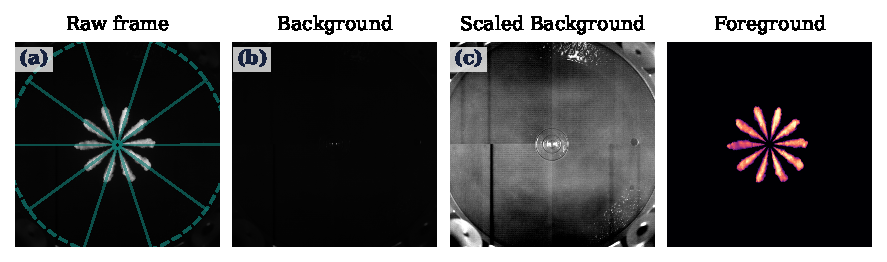
\includegraphics[width=0.98\linewidth]{images/fig_mie_preproc_background.png}
\caption{预处理中间结果：原始帧、背景估计和对数减背景前景。}
\label{fig:mie-preproc-background}
\end{figure}

\subsubsection{CUDA 后端上的超高效 Sobel 高通}

Sobel 高通阶段仍按英文稿中的做法，直接在整段视频张量上计算梯度幅值，并把结果保留在 CuPy 后端中，以获得适合后续 plume 几何分析的边缘占优表示。

\begin{figure}[t]
\centering

\includegraphics[width=0.98\linewidth]{images/fig_mie_preproc_sobel.png}
\caption{前景图、Sobel 幅值图与稳健缩放高通表示。}
\label{fig:mie-preproc-sobel}
\end{figure}

\subsubsection{将角向密度视为极坐标重采样}

角向密度通过围绕喷嘴中心的极坐标重采样获得，从二维图像得到一维角向占据信号，以便后续按喷孔周期结构进行配准。

\subsubsection{基于 FFT 的自适应旋转对齐}

通过读取角向累计信号在 plume 数对应谐波上的相位，自动估计旋转偏移，并构造每个 plume 的目标方向。

\begin{figure}[t]
\centering

\includegraphics[width=0.98\linewidth]{images/fig_angular_occupancy.png}
\caption{角向密度、时间累计剖面、FFT 谐波和占据角度 mask。}
\label{fig:angular-occupancy}
\end{figure}

\subsubsection{逆仿射映射与 plume strip 提取}

对每个 plume 构造逆仿射映射，把喷雾重采样到统一的局部 strip 坐标中，方便后续对每个 plume 施加统一度量。

\begin{figure}[t]
\centering

\includegraphics[width=0.98\linewidth]{images/fig_efficient_rotation.png}
\caption{逆仿射重映射阶段可视化。}
\label{fig:efficient-rotation}
\end{figure}

\subsubsection{基于对齐 plume strip 的稳健 CDF 穿深}

穿深估计使用累积分布前沿而不是最前像素，降低对孤立前沿像素和破碎小块的敏感性。

\subsubsection{边界指标与几何代理量}

除穿深外，工作流还提取面积、极坐标穿深、类体积代理量和锥角代理量，用作更丰富的喷雾几何状态描述。

\begin{figure}[t]
\centering

\includegraphics[width=0.98\linewidth]{images/fig_mie_metrics_summary.png}
\caption{plume 对齐和二值化后得到的多种几何输出。}
\label{fig:mie-metrics-summary}
\end{figure}

\subsection{\codepath{MLP/fit_raw_data.py} 中的轨迹清洗与降阶拟合}

这一阶段清洗原始轨迹、对齐延迟、剔除不合理跳变，并用平滑的双分支模型拟合每条轨迹。其作用既是平滑压缩，也是面向删失的目标构造步骤，用于为后续网络训练提供更稳定、可微且更适合监督学习的穿深目标。

\subsection{\codepath{MLP/median_penetration_MSE.ipynb} 中的 Stage-1 确定性基线}

Stage 1 在每个工况组中选取 5 ms 处最接近组中位数的代表性轨迹，以 9 个工况和时间特征为输入，用 MSE 加上单调性与凹性软约束训练一个双输出 MLP。当前归档结果显示该阶段已经保存了完整 checkpoint、loss 日志和 scaler 状态，是最完整的可部署工件。

\subsection{\codepath{MLP/median_penetration_NLL.ipynb} 中的 Stage-2 异方差扩展}

Stage 2 从 stage 1 warm-start，扩展到全部通过远时刻筛选的拟合轨迹，并用异方差高斯 NLL 同时学习均值和方差。它在归档日志中表现良好，但由于缺失专门的 stage-2 checkpoint 和部分中间训练目录，目前只能算作部分完成的结果。

\subsection{Warm-start 原始 CDF 细化与保守蒸馏}

第三阶段的设计动机与英文稿一致：早期 raw CDF 轨迹比拟合曲线更能保留真实瞬态，但晚期又受到右删失污染，因此需要把可靠的 raw 早期监督与教师模型提供的保守延拓结合起来，而不是直接把消失的晚期观测当成硬标签。

\begin{figure}[t]
\centering
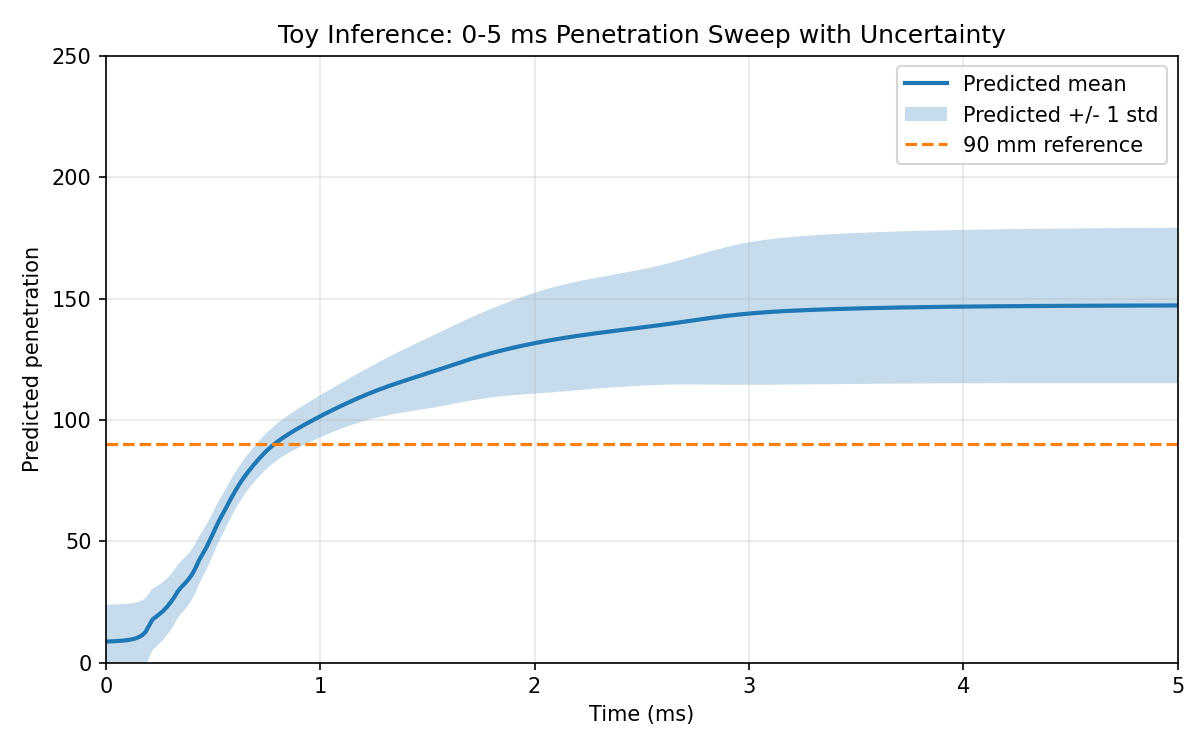
\includegraphics[width=0.82\linewidth]{images/stage2_toy_inference_2000bar_5bar.png}
\caption{代表性 stage-2 toy inference，可见早期仍受拟合先验影响。}
\label{fig:stage2-toy-inference-early-time}
\end{figure}

\subsection{原型推理 notebook}

\codepath{MLP/toy_inference_from_run.ipynb} 用于从保存的 run 目录加载模型和 scaler，生成均值/标准差曲线，并与简化几何掩膜叠加。它证明了推理链是可打通的，但当前仍只是原型。

\section{结果}

\subsection{已提取与清洗的轨迹资产}

当前工作区包含多个 campaign 文件夹以及 295 个 clean fitted CSV 文件，说明图像处理和 clean-fit 阶段已经形成了一套可审计的数据资产。

\begin{figure}[t]
\centering
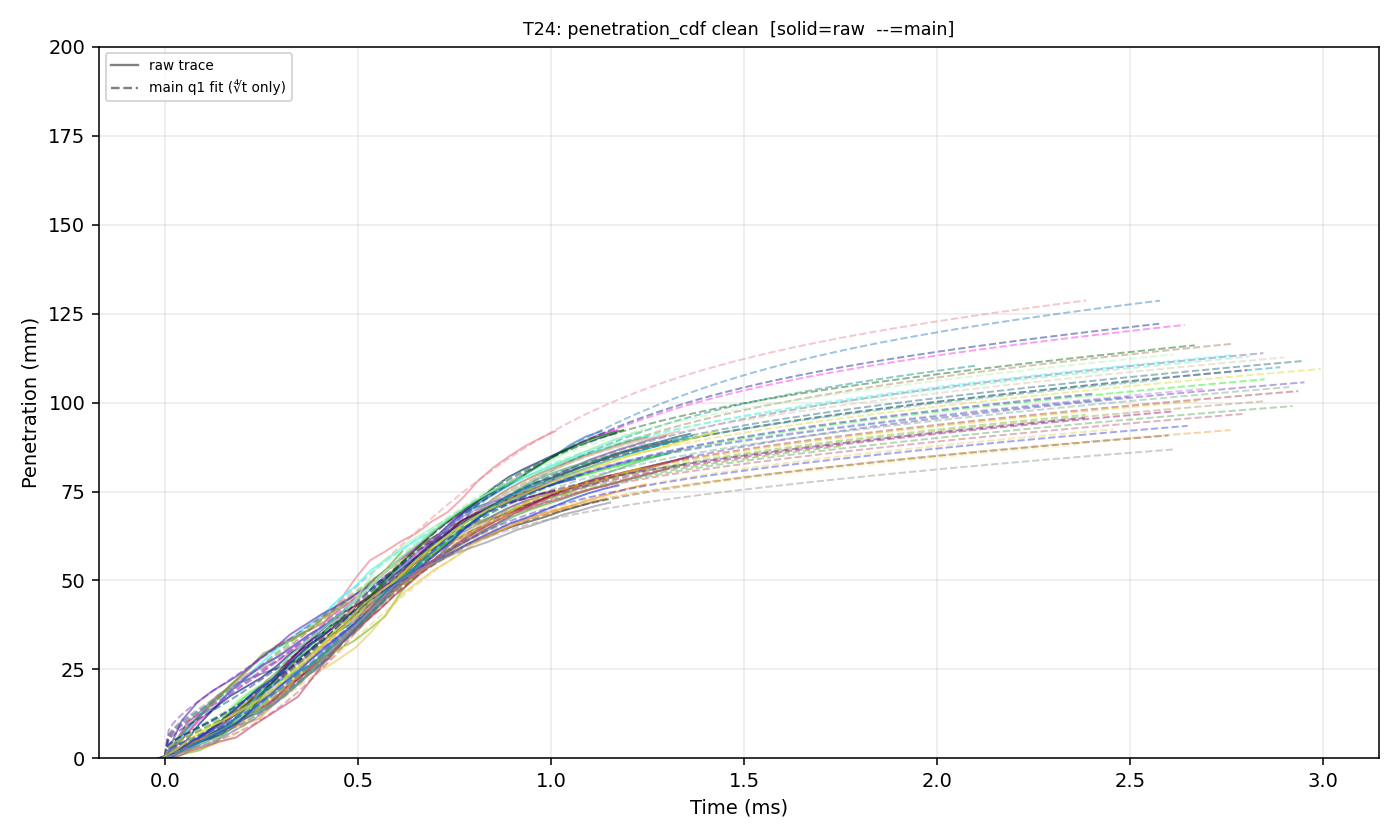
\includegraphics[width=0.92\linewidth]{images/representative_clean_fit.png}
\caption{代表性的 clean trajectory 与 fitted curve 图。}
\label{fig:clean-fit-example}
\end{figure}

\subsection{Stage-1 基线模型}

Stage 1 的归档 run 目录包含完整 checkpoint、配置和训练日志。最佳归档验证 MSE 为 23.26，出现在第 429 个 epoch。这是当前最完整、最明确的 surrogate 结果。

\begin{figure}[t]
\centering
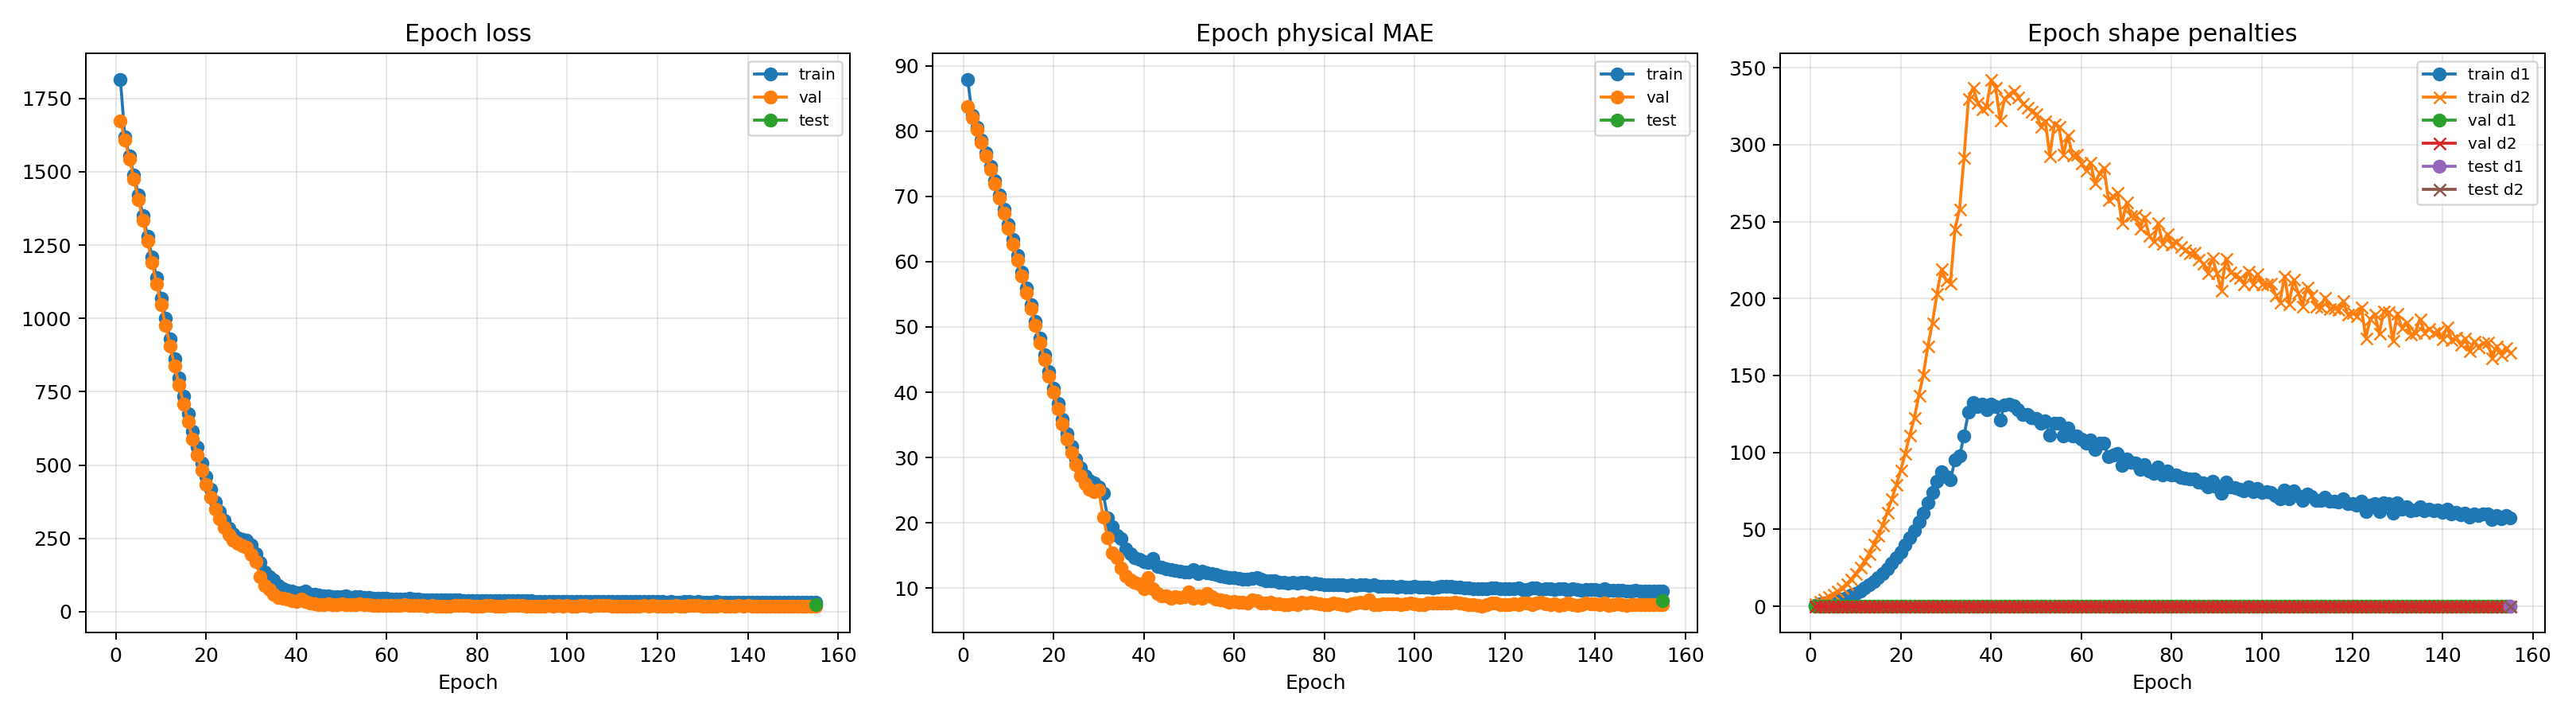
\includegraphics[width=0.92\linewidth]{images/stage1_loss_curves.png}
\caption{归档的 stage-1 loss 曲线。}
\label{fig:stage1-loss}
\end{figure}

\subsection{Stage-2 不确定性感知扩展}

Stage 2 的归档日志显示最佳验证 NLL 为 2.449，出现在第 570 个 epoch。它说明异方差扩展在 warm-start 和重筛选数据条件下具有可行性，但由于缺少完整打包模型，当前仍应视为部分结果。

\begin{figure}[t]
\centering
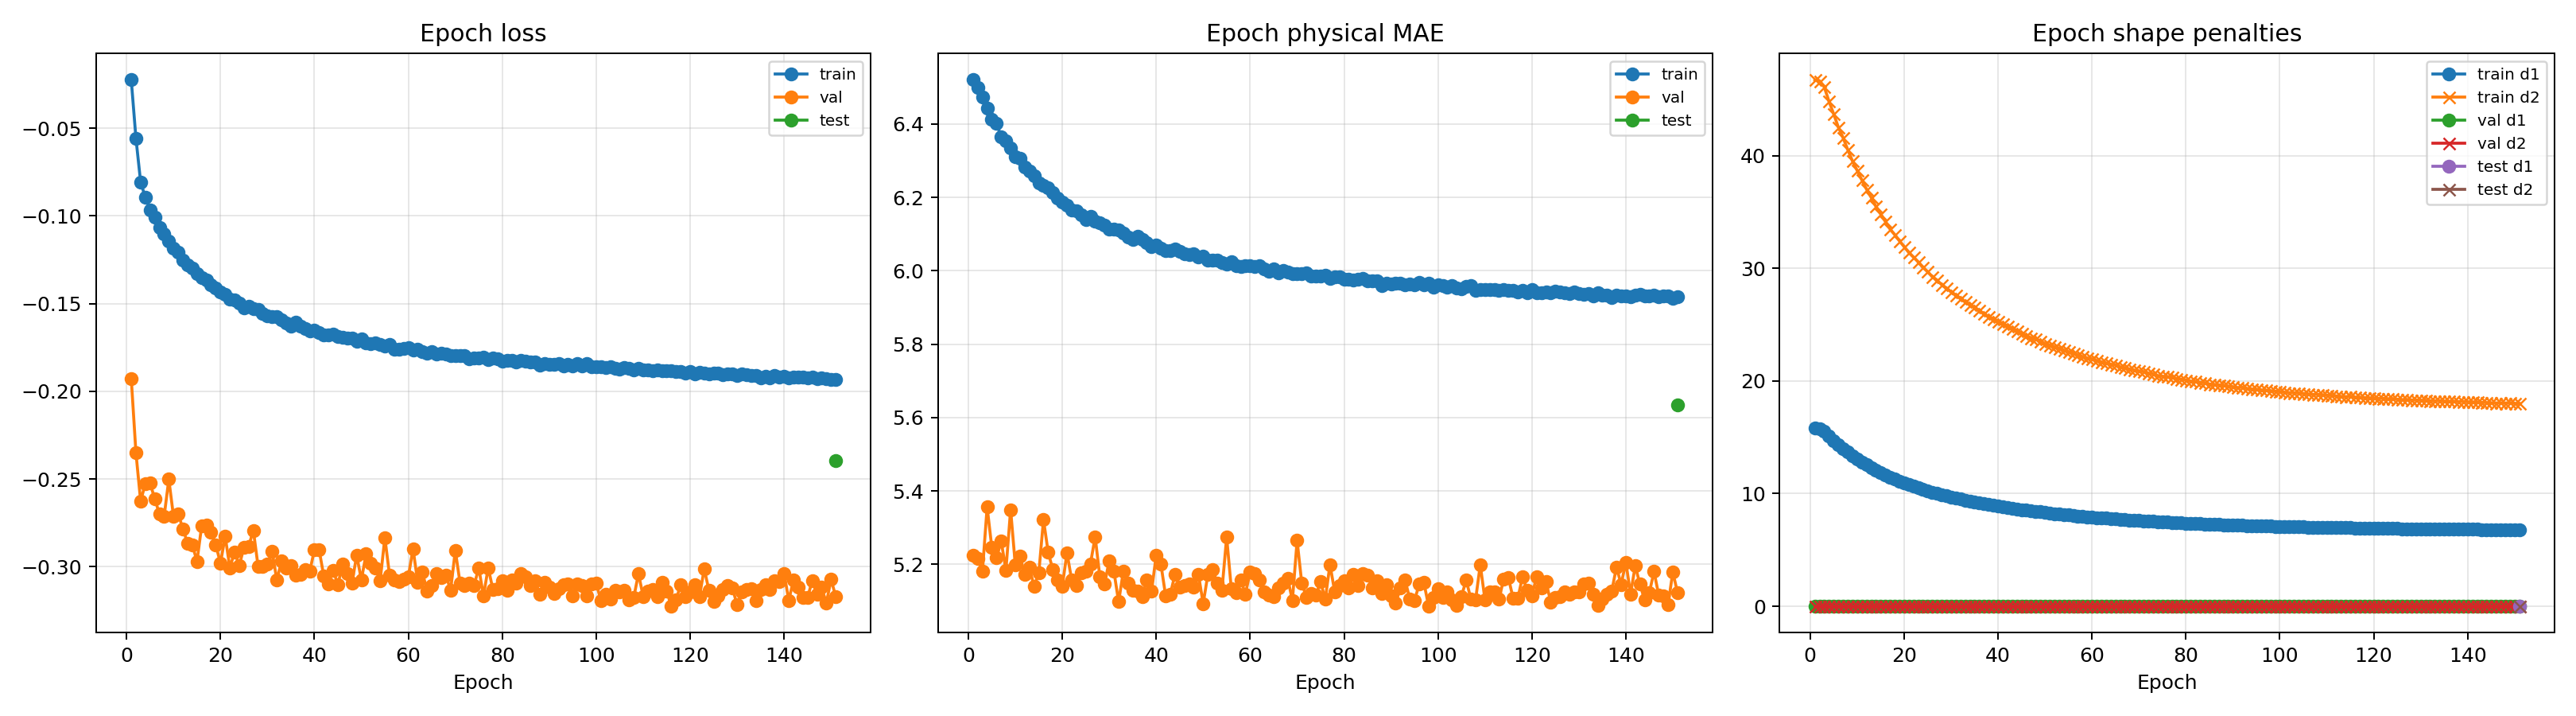
\includegraphics[width=0.92\linewidth]{images/stage2_loss_curves.png}
\caption{归档的 stage-2 loss 曲线。}
\label{fig:stage2-loss}
\end{figure}

\subsection{原型推理 notebook}

原型 notebook 可以加载归档运行元数据，生成均值/标准差曲线并与 wall/cylinder mask 做简单叠加。但当前证据只足以支撑软件集成概念验证，尚不足以支撑完整撞壁分析框架。

\begin{table}[t]
\centering
\begin{tabular}{|L{0.20\linewidth}|L{0.18\linewidth}|L{0.20\linewidth}|L{0.20\linewidth}|}
\hline
阶段 & 数据证据 & 最佳归档验证结果 & 当前状态 \\
\hline
图像处理与拟合 & \codepath{MLP/synthetic_data} 下有 10 个 campaign 文件夹和 295 个 clean fitted CSV & 已有代表性 clean/fitted trajectory 图 & 已完成且可审计 \\
\hline
Stage 1 MSE 基线 & 归档 notebook 输出：589 行，划分为 413/88/88 & 第 429 个 epoch 的验证 MSE 为 23.26 & 已完成并保存 checkpoint \\
\hline
Stage 2 NLL 扩展 & 归档 notebook 输出：21,177 行，划分为 14,825/\allowbreak 3,176/\allowbreak 3,176 & 第 570 个 epoch 的验证 NLL 为 2.449 & 部分结果；当前运行目录中无保存的 stage-2 checkpoint \\
\hline
原型推理 & 来自 \codepath{MLP/toy_inference_from_run.ipynb} 的归档 notebook 输出 & 均值/标准差预测图及简单重叠计算 & 仅为原型，不是已验证产品 \\
\hline
\end{tabular}
\caption{已完成阶段与部分完成阶段的证据汇总。}
\label{tab:model-summary}
\end{table}

\subsection{结果边界与可复现性状态}

当前最强的可复现证据来自提取、清洗和 stage-1 基线归档；最薄弱之处在于 stage-2 缺少专门 checkpoint 和中间训练目录。因此，本文在结果表述上对 stage 2 保持边界意识，不把它写成已完全闭环的部署模型。

\section{结论}

本文建立了一条从高速 Mie 散射喷雾视频到穿深导向工程观测量、再到归档 surrogate 模型的证据化工作流。当前完成度最高的贡献包括：\texttt{GUI.py} 中的人工标定、\texttt{main.py} 中的批量 plume 特征提取、\codepath{MLP/fit_raw_data.py} 中的 clean-fit 阶段，以及带完整 checkpoint 的 stage-1 确定性穿深模型。

Stage-2 异方差扩展很有前景，但在当前工作区中仍未打包完整。原型推理 notebook 则说明模型加载、曲线可视化和简单几何叠加都已经可行，但经过验证的碰撞预测与完整部署仍属于未来工作。

\thesisbibliography

\ifXeTeX
\else
\end{CJK*}
\fi
\end{document}
